\documentclass[11pt]{article}
\usepackage[utf8]{inputenc}
\usepackage[spanish,es-tabla,es-nodecimaldot]{babel}

% Paquetess

\usepackage{amsmath}
\usepackage{amsthm}
\usepackage{amsfonts}
\usepackage{amssymb}
\usepackage{makeidx}
\usepackage{graphicx}
\usepackage{lmodern}
\usepackage[dvipsnames]{xcolor} 
\usepackage{fancyhdr}
\usepackage{geometry}
\usepackage{lastpage}		
\usepackage{array}			 % Para fjar tamaño de columnas
\usepackage{tikz}
\usepackage{subcaption}
\usepackage{caption}
\usepackage{pgfplots} % Para controlar la perspectiva
\RequirePackage{siunitx}
\usepackage{extramarks} % Para poder usar firstleftmarks
\usepackage[version=4]{mhchem} % Para poder usar formulas de reacciones nucleares
\usepackage{chemfig}
\usepackage{xcolor}
\RequirePackage[most]{tcolorbox}
\usepackage{enumitem}
\usepackage{physics}
%\usepackage{background}
\usepackage{eso-pic} % Para insertar imágenes de fondo específicas
\usepackage[absolute,overlay]{textpos} % Paquete para colocar elementos en posiciones absolutas
\usepackage{wrapfig}



\newtcolorbox{mybox}{colback=black!5!white,
	colframe=black!75!black}

\newtcolorbox{Anotacion}{colback=red!5!white,
	colframe=red!75!red}


%##############################################################################
%######### Ponemos el decimal con . ###########################################
%##############################################################################

\sisetup{output-decimal-marker={.},
	% exponentes ------------------------
	exponent-mode=threshold,
	exponent-thresholds=-3:2, % non usar exponentes 10^{-2,-1, 0, 1}
	% redondear -------------------------
	% round-mode=figures, % cifras sig
	% round-mode=places, % cantos decimales
	round-mode=uncertainty, % cifras sig da incerteza (necesario usar erro)
	round-precision=2,
	uncertainty-mode = separate,
	print-unity-mantissa=false,
	% unidades --------------------------
	inter-unit-product = \ensuremath{{}\cdot{}}, % separacion entre unidades
	% per-mode=power-positive-first, % so furrula con metodo interpretado puro
	inline-per-mode=single-symbol,
	display-per-mode=fraction,
}

%##############################################################################
%######### Para codigo python #################################################
%##############################################################################

\definecolor{codegreen}{rgb}{0,0.6,0}
\definecolor{codegray}{rgb}{0.5,0.5,0.5}
\definecolor{codepurple}{rgb}{0.58,0,0.82}

\usepackage{listings}


%\lstdefinestyle{mystyle}{	backgroundcolor=\color{backcolour},   	commentstyle=\color{codegreen},	keywordstyle=\color{magenta},	numberstyle=\tiny\color{codegray},	stringstyle=\color{codepurple},	basicstyle=\ttfamily\footnotesize,	breakatwhitespace=false,         	breaklines=true,                 	captionpos=b,                    	keepspaces=true,                 	numbers=left,                    	numbersep=5pt,                  	showspaces=false,                	showstringspaces=false,	showtabs=false,                  	tabsize=2}

%\lstset{style=mystyle}
%\usepackage{background}     % Para manejar el fondo


%##############################################################################
%######### Tipo de fuente #################################################
%##############################################################################

\usepackage{newtxtext,newtxmath} % Cambia la fuente (pero mola)
%\usepackage{kpfonts}

%\usepackage{helvet} 
%\renewcommand{\familydefault}{\sfdefault}.

%\usepackage{fontspec} % Paquete necesario para seleccionar fuentes
%\setmainfont{Verdana} % Cambia la fuente principal a Verdana


%##############################################################################
%######### Geometría #################################################
%##############################################################################

\geometry{a4paper, total={152mm,237mm}, left=31mm, top=30mm}



%##############################################################################
%######### Formatos capítulo #################################################
%##############################################################################

%\usepackage[lmodern]{quotchap}
%\usepackage[options]{fncychap}
% Configuración de la imagen de fondo solo para la portada



%##############################################################################
%######### Hiperreferenias #################################################
%##############################################################################


\usepackage[colorlinks=true, linkcolor=RoyalBlue, citecolor=ForestGreen, urlcolor=BrickRed]{hyperref} % Crea las
\usepackage[nameinlink]{cleveref}
\crefname{figure}{Fig.}{Figs.}

%##############################################################################
%######### Formato de pagina #################################################
%##############################################################################

\pagestyle{fancy}
\fancyhf{} % Limpia encabezados y pies
\fancyhead[L]{\small \textbf{Memoria Resistividad de Placas}}    % Encabezado izquierdo
\fancyhead[R]{\small \textbf{Daniel Vázquez Lago}}     % Encabezado derecho
\fancyfoot[C]{\thepage}      % Pie de página centrado con el número de página
\renewcommand{\headrulewidth}{0.4pt}  % Grosor de la línea del encabezado
\renewcommand{\footrulewidth}{0pt}    % Sin línea en el pie



%##############################################################################
%#########  Modificar caption #################################################
%##############################################################################

\usepackage[font=small, justification=centering]{caption}  % Configura las captions



%##############################################################################
%######### Comandos propios #################################################
%##############################################################################


\newcommand{\parentesis}[1]{\left( #1  \right)}
\newcommand{\parciales}[2]{\frac{\partial #1}{\partial #2}}
\newcommand{\pparciales}[2]{\parentesis{\parciales{#1}{#2}}}
\newcommand{\ccorchetes}[1]{\left[ #1  \right]}
\newcommand{\D}{\mathrm{d}}
\newcommand{\derivadas}[2]{\frac{\D #1}{\D #2}}

\newcommand{\tquad}{\quad \quad \quad}
%\newcommand{\vnabla}{\vec{\nabla}}

\newcommand{\Ocal}{\mathcal{O}}
\newcommand{\Jcal}{\mathcal{J}}
\newcommand{\Mcal}{\mathcal{M}}
\newcommand{\Fcal}{\mathcal{F}}
\newcommand{\Hcal}{\mathcal{H}}
\newcommand{\Ecal}{\mathcal{E}}
\newcommand{\Ncal}{\mathcal{N}}

\newcommand{\cmm}{\text{cm}^{-1}}
\newcommand{\fcc}{\textit{fcc}}
\newcommand{\bcc}{\textit{bcc}}
\renewcommand{\sc}{\textit{sc}}
\newcommand{\hcp}{\textit{hcp}}


\newcommand{\PZB}{\text{{\tiny PZB}}}
\newcommand{\gap}{\text{{\tiny gap}}}
\newcommand{\SZB}{\text{{\tiny SZB}}}
\newcommand{\inicial}{\text{{\tiny inicial}}}
\newcommand{\final}{\text{{\tiny final}}}
\newcommand{\atomico}{\text{{\tiny atómico}}}

\newcommand{\arctanh}{\text{{arctanh}}}



\newcommand{\Namas}{\text{Na}^+}
\newcommand{\Clmenos}{\text{Cl}^-}

\newcommand{\cm}{\text{cm}}
\newcommand{\eV}{\text{eV}}

\newcommand{\arr}{\text{arr}}
\newcommand{\diff}{\text{diff}}

\newcommand{\er}{$^{\text{er}}$}
\newcommand{\cte}{\text{cte}}
\newcommand{\expo}{\text{exp}}
\newcommand{\simu}{\text{simu}}


% Comandos vectoriales

\newcommand{\an}{\mathbf{a}}
\newcommand{\bn}{\mathbf{b}}
\newcommand{\dn}{\mathbf{d}}
\newcommand{\fn}{\mathbf{f}}
\newcommand{\jn}{\mathbf{j}}
\newcommand{\kn}{\mathbf{k}}
\newcommand{\pn}{\mathbf{p}}
\newcommand{\qn}{\mathbf{q}}
\newcommand{\rn}{\mathbf{r}}
\newcommand{\sn}{\mathbf{s}}
\newcommand{\un}{\mathbf{u}}
\newcommand{\vn}{\mathbf{v}}
\newcommand{\xn}{\mathbf{x}}
\newcommand{\wn}{\mathbf{w}}
\newcommand{\yn}{\mathbf{y}}
\newcommand{\qndot}{\dot{\qn}}

\newcommand{\alphan}{\boldsymbol{\alpha}}
\newcommand{\sigman}{\boldsymbol{\sigma}}
\newcommand{\pin}{\boldsymbol{\pi}}
\newcommand{\rhon}{\boldsymbol{\rho}}
\newcommand{\epsilonn}{\boldsymbol{\epsilon}}
\newcommand{\omegan}{\boldsymbol{\omega}}
\newcommand{\mun}{\boldsymbol{\mu}}



\newcommand{\An}{\mathbf{A}}
\newcommand{\Bn}{\mathbf{B}}
\newcommand{\En}{\mathbf{E}}
\newcommand{\Fn}{\mathbf{F}}
\newcommand{\Jn}{\mathbf{J}}
\newcommand{\Hn}{\mathbf{H}}
\newcommand{\Gn}{\mathbf{G}}
\newcommand{\Kn}{\mathbf{K}}
\newcommand{\Ln}{\mathbf{L}}
\newcommand{\Mn}{\mathbf{M}}
\newcommand{\Pn}{\mathbf{P}}
\newcommand{\Rn}{\mathbf{R}}
\newcommand{\Sn}{\mathbf{S}}
\newcommand{\Tn}{\mathbf{T}}
\newcommand{\In}{\mathbf{1}}
\newcommand{\Encal}{\boldsymbol{\mathcal{E}}}

\newcommand{\hnn}{\hat{\mathbf{n}}}
\newcommand{\hnr}{\hat{\mathbf{r}}}
\newcommand{\hnz}{\hat{\mathbf{z}}}
\newcommand{\hnv}{\hat{\mathbf{v}}}
\newcommand{\hnx}{\hat{\mathbf{x}}}
\newcommand{\hny}{\hat{\mathbf{y}}}
\newcommand{\hnu}{\hat{\mathbf{u}}}
\newcommand{\hnR}{\hat{\mathbf{R}}}
\newcommand{\hnp}{\hat{\mathbf{p}}}
\newcommand{\hnk}{\hat{\mathbf{k}}}
\newcommand{\hni}{\hat{\mathbf{i}}}
\newcommand{\hnj}{\hat{\mathbf{j}}}
\renewcommand{\hnk}{\hat{\mathbf{k}}}

 
\title{Memoria Tecnicas IV Sólido: Resistividad de Placas}
\author{Daniel Vázquez Lago}
\date{\today}




\begin{document}

\maketitle

\tableofcontents

\newpage

\section{Objetivos}

El principal objetivo es determinar la resisitivdad eléctrica del material de la placa de espesor 1 mm, y luego identificar el metal. 

\section{Procedimiento a la medida}

Esta es la parte puramente experimental. Lo que hacemos es inyectar una corriente por dos terminales cualquiera (1,2,3,4), imágen \textcolor{red}{[¿?]}, midiendo la diferencia de voltaje por otras dos. Nostros realizamos 4 medidas de Intensidad-Voltaje (tal que $I\leq 4$ A y $V\leq 1$ mV) en 6 diferentes disposiciones. Realizar 4 medidas, que nosotros tomamos desde 1.5 A a 3.0 A con un intervalo de 0.5 A, es suficiente para comprobar que efectivamente es un material óhmico, que es la única exigencia que vamos a realizar para el análisis posterior. Dado que el cálculo de la resistividad se realiza con un solo valor del voltaje para cada disposición no será un problema tener pocas medidas (al memos en comparación con otras prácticas). 

Como relaizamos la digitalización o la simulación es un, ciertamente, innecesario, ya que todo lo que realizamos está en el guión de la práctica. 

\section{Calculo de la resistivdad del material}

Como ya hemos indicado, nosotros vamos a medir voltajes para una entrada particular de intensidad, queriendo calcular la resisitivdad del material, por lo que la información importante será $(V_{\exp},\sigma_{\exp})$, siendo $\sigma_{\exp}$ la que queremos calcular. Los valores que nos va a dar la simulación son pares de $(V_{\simu},\sigma_{\simu}$) siendo la intensidad $I_{\exp}$ y $I_{\simu}$ iguales, en una experimental y en otra un parámetro que introducimos a mano. Dado que la ley de Ohm $V\varpropto \rho = 1 / \sigma$ que hemos comprobado que el material sigue:, podemos suponer que $V\times \sigma = \cte$, y por tanto se debe verificar que: 

\begin{equation}
	V_{\exp} \times \sigma_{\exp} = V_{\simu} \times \sigma_{\simu}
\end{equation}

\section{Resultados}

\subsection{Material óhmico}

\begin{figure}[h!]\centering
\begin{subfigure}[b]{0.49\textwidth}
	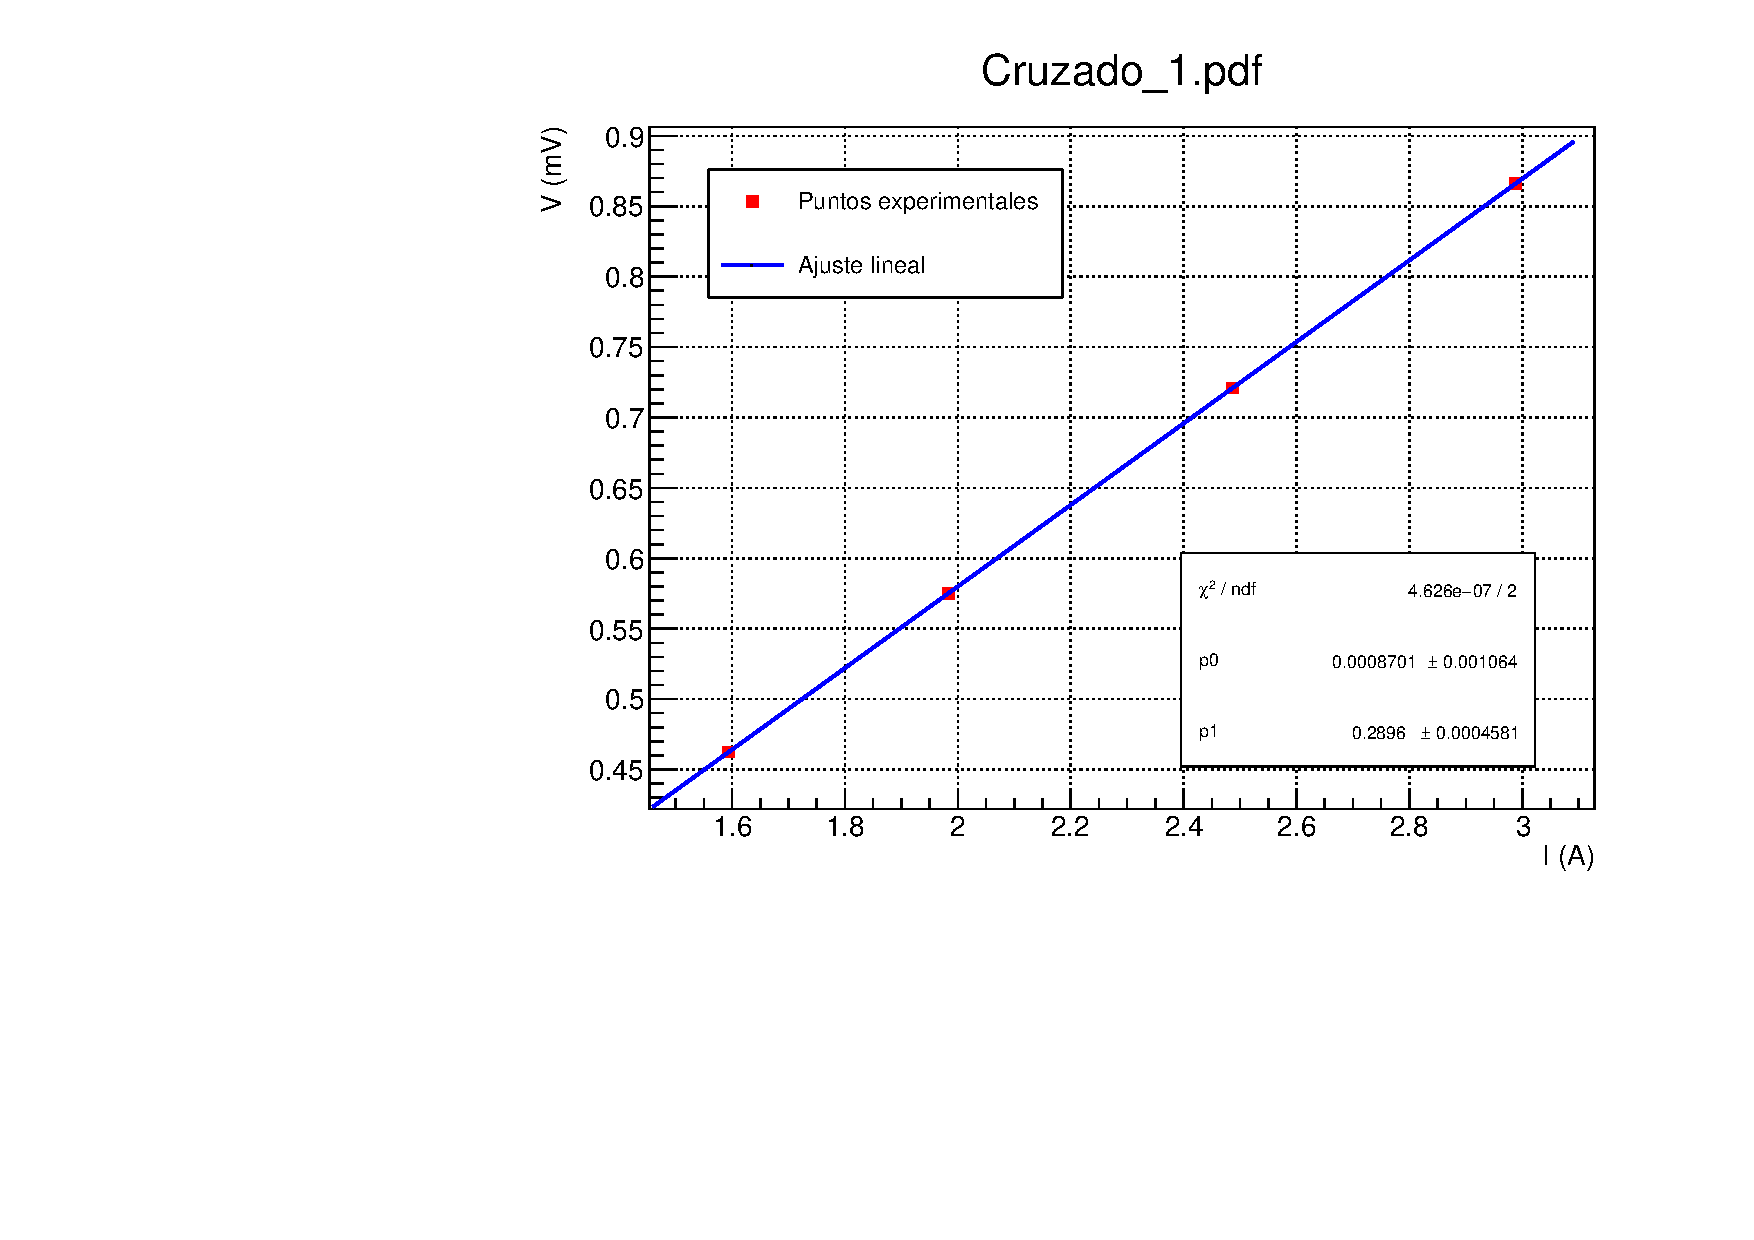
\includegraphics[width=1.05\linewidth]{Programas/Cruzado_1.pdf}
\end{subfigure} \hfill
\begin{subfigure}[b]{0.49\textwidth}
	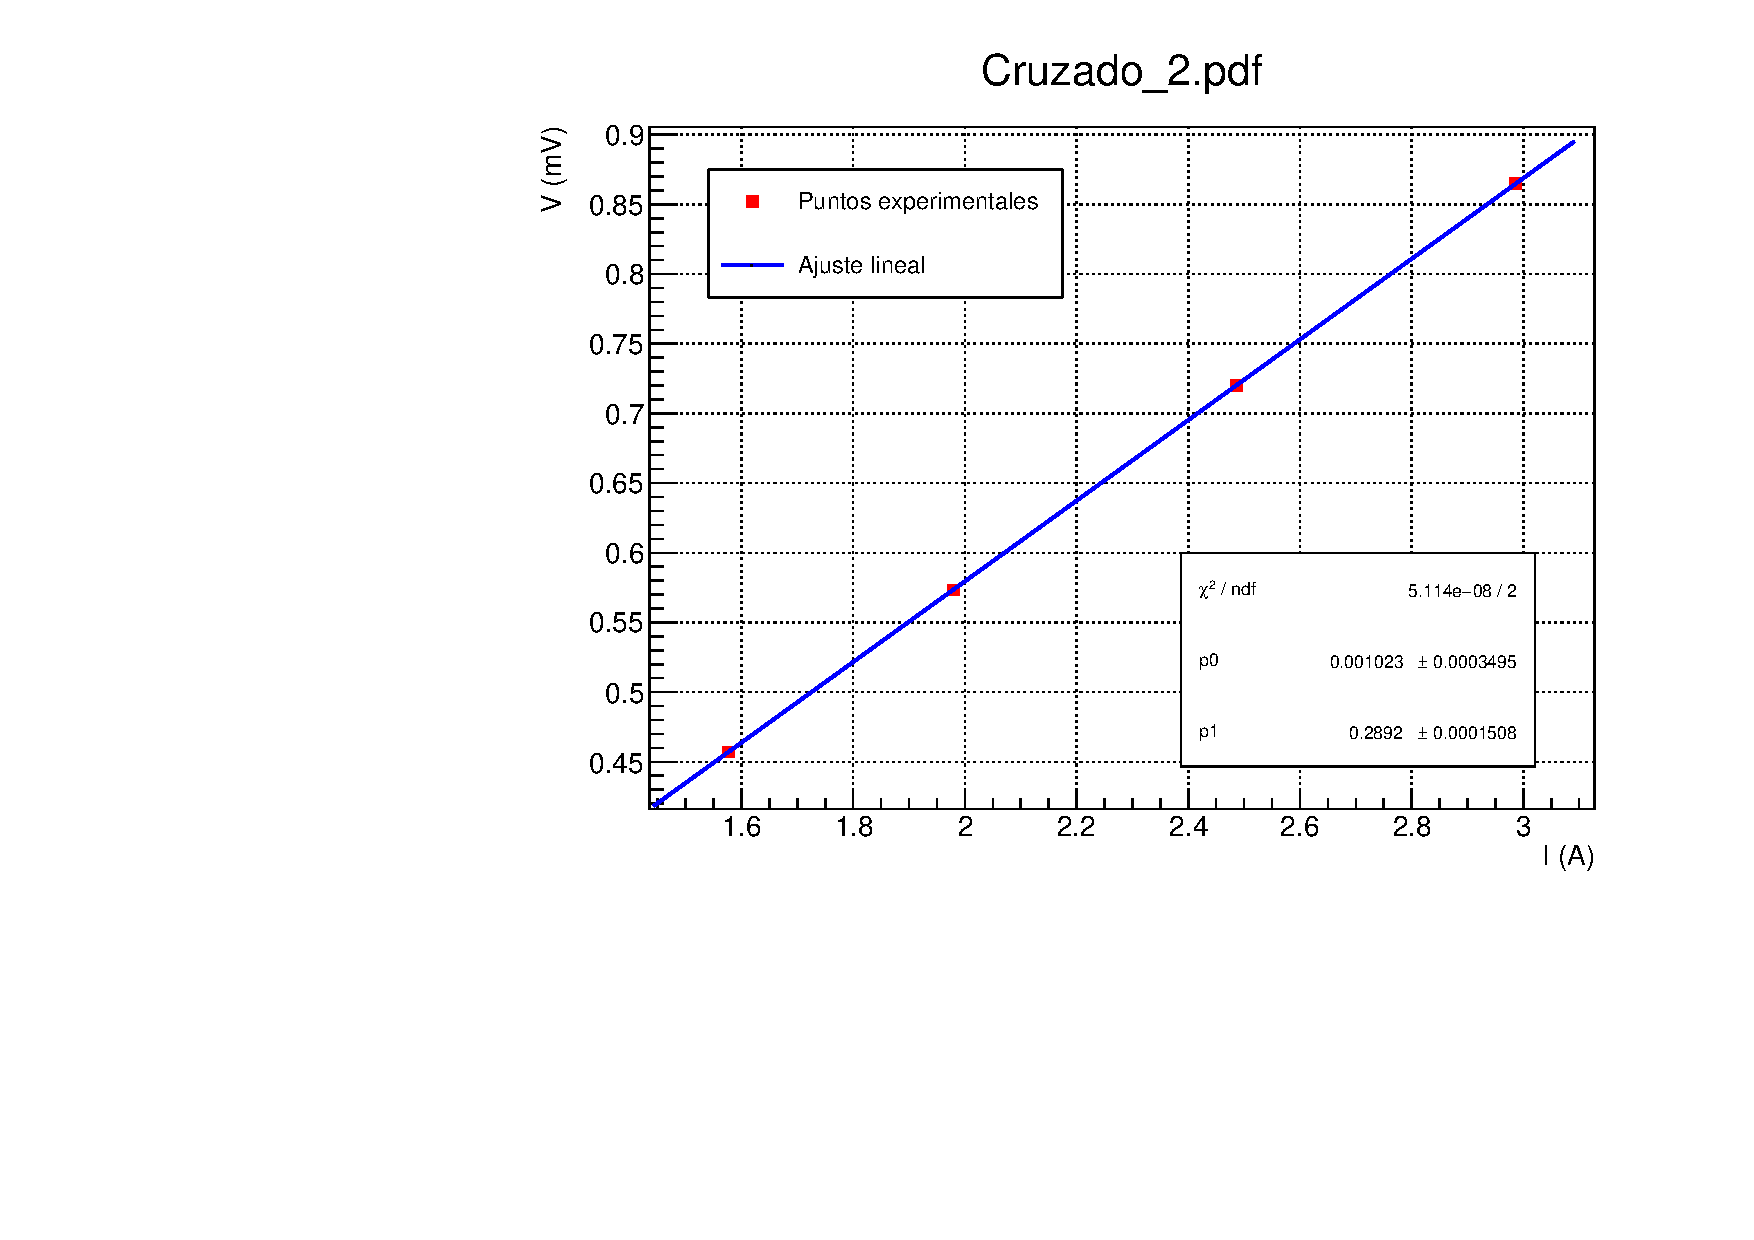
\includegraphics[width=1.05\linewidth]{Programas/Cruzado_2.pdf}
\end{subfigure}
\end{figure}
\begin{figure}[h!]\centering
\begin{subfigure}[b]{0.49\textwidth}
	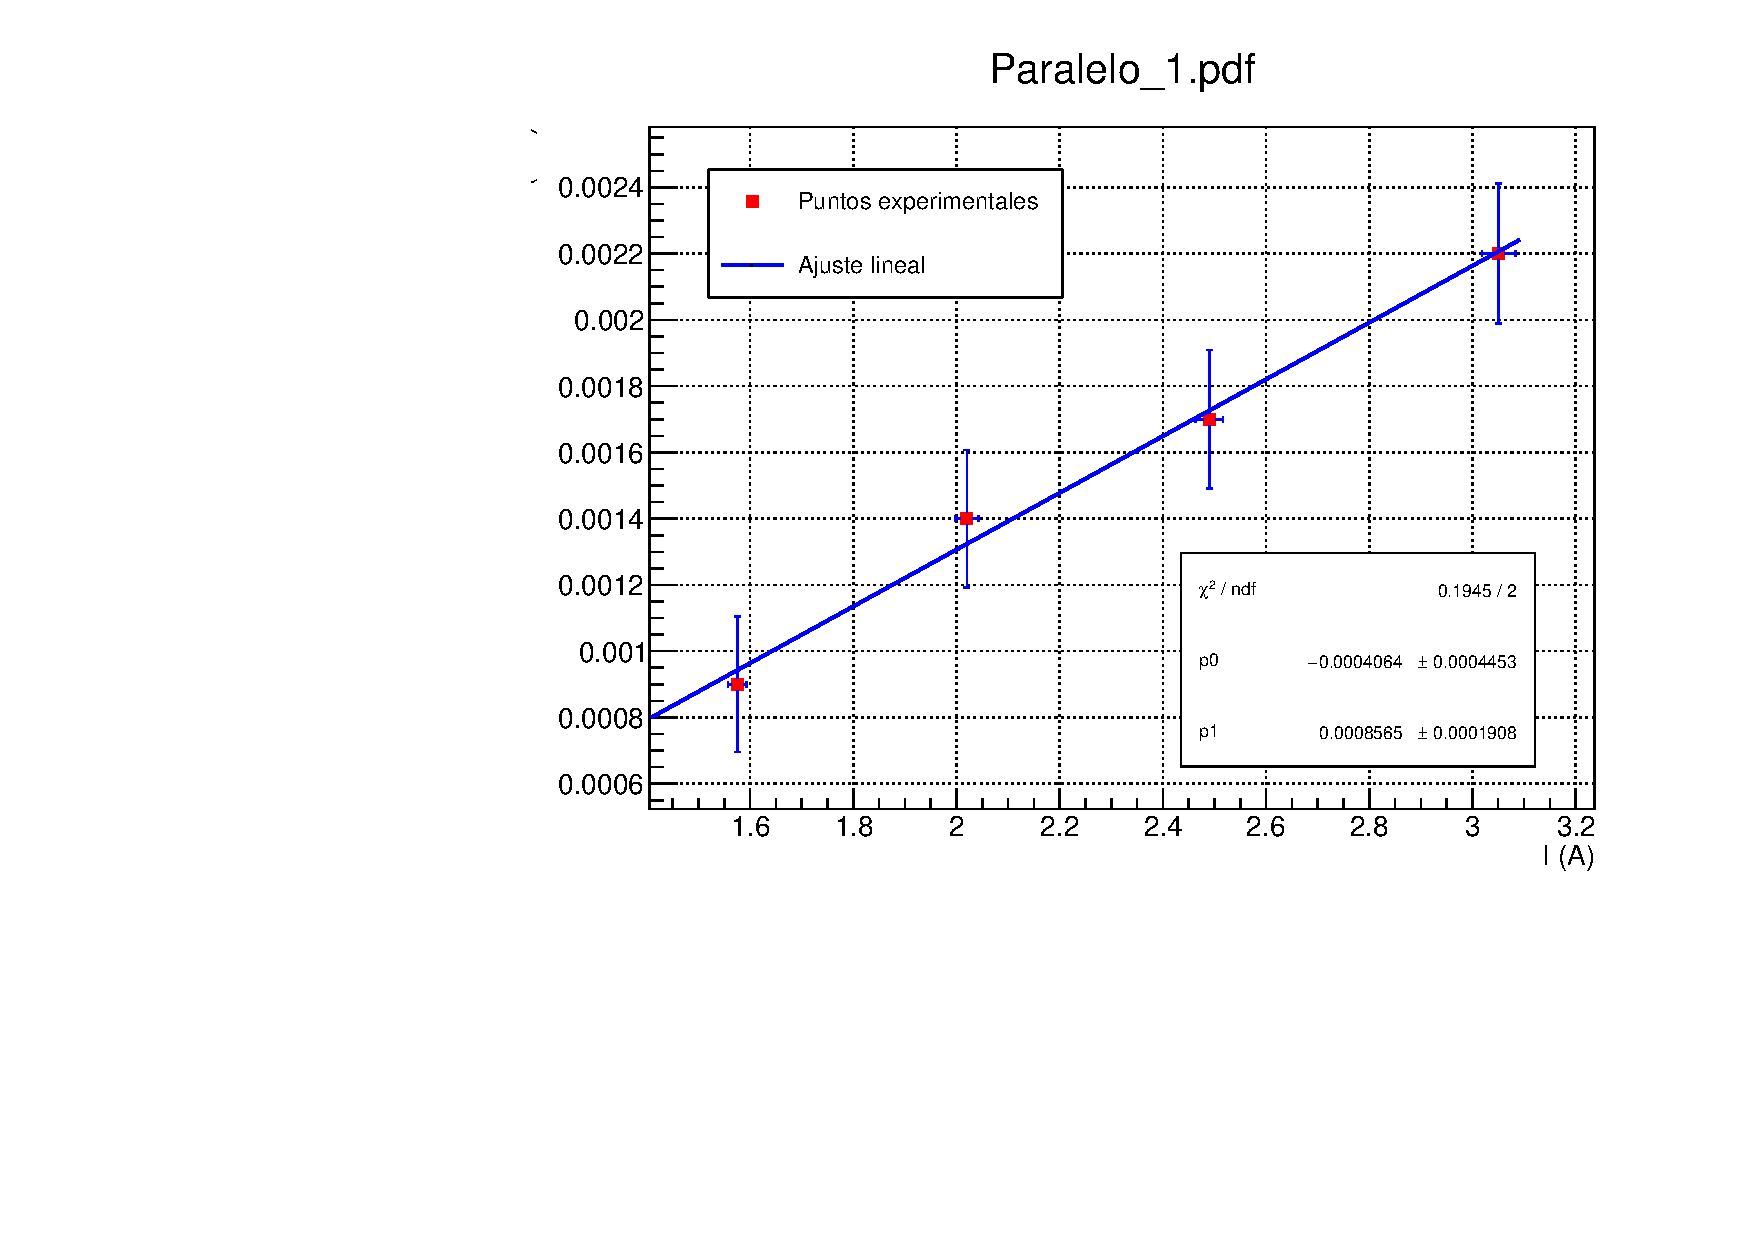
\includegraphics[width=1.05\linewidth]{Programas/Paralelo_1.pdf}
\end{subfigure} \hfill
\begin{subfigure}[b]{0.49\textwidth}
	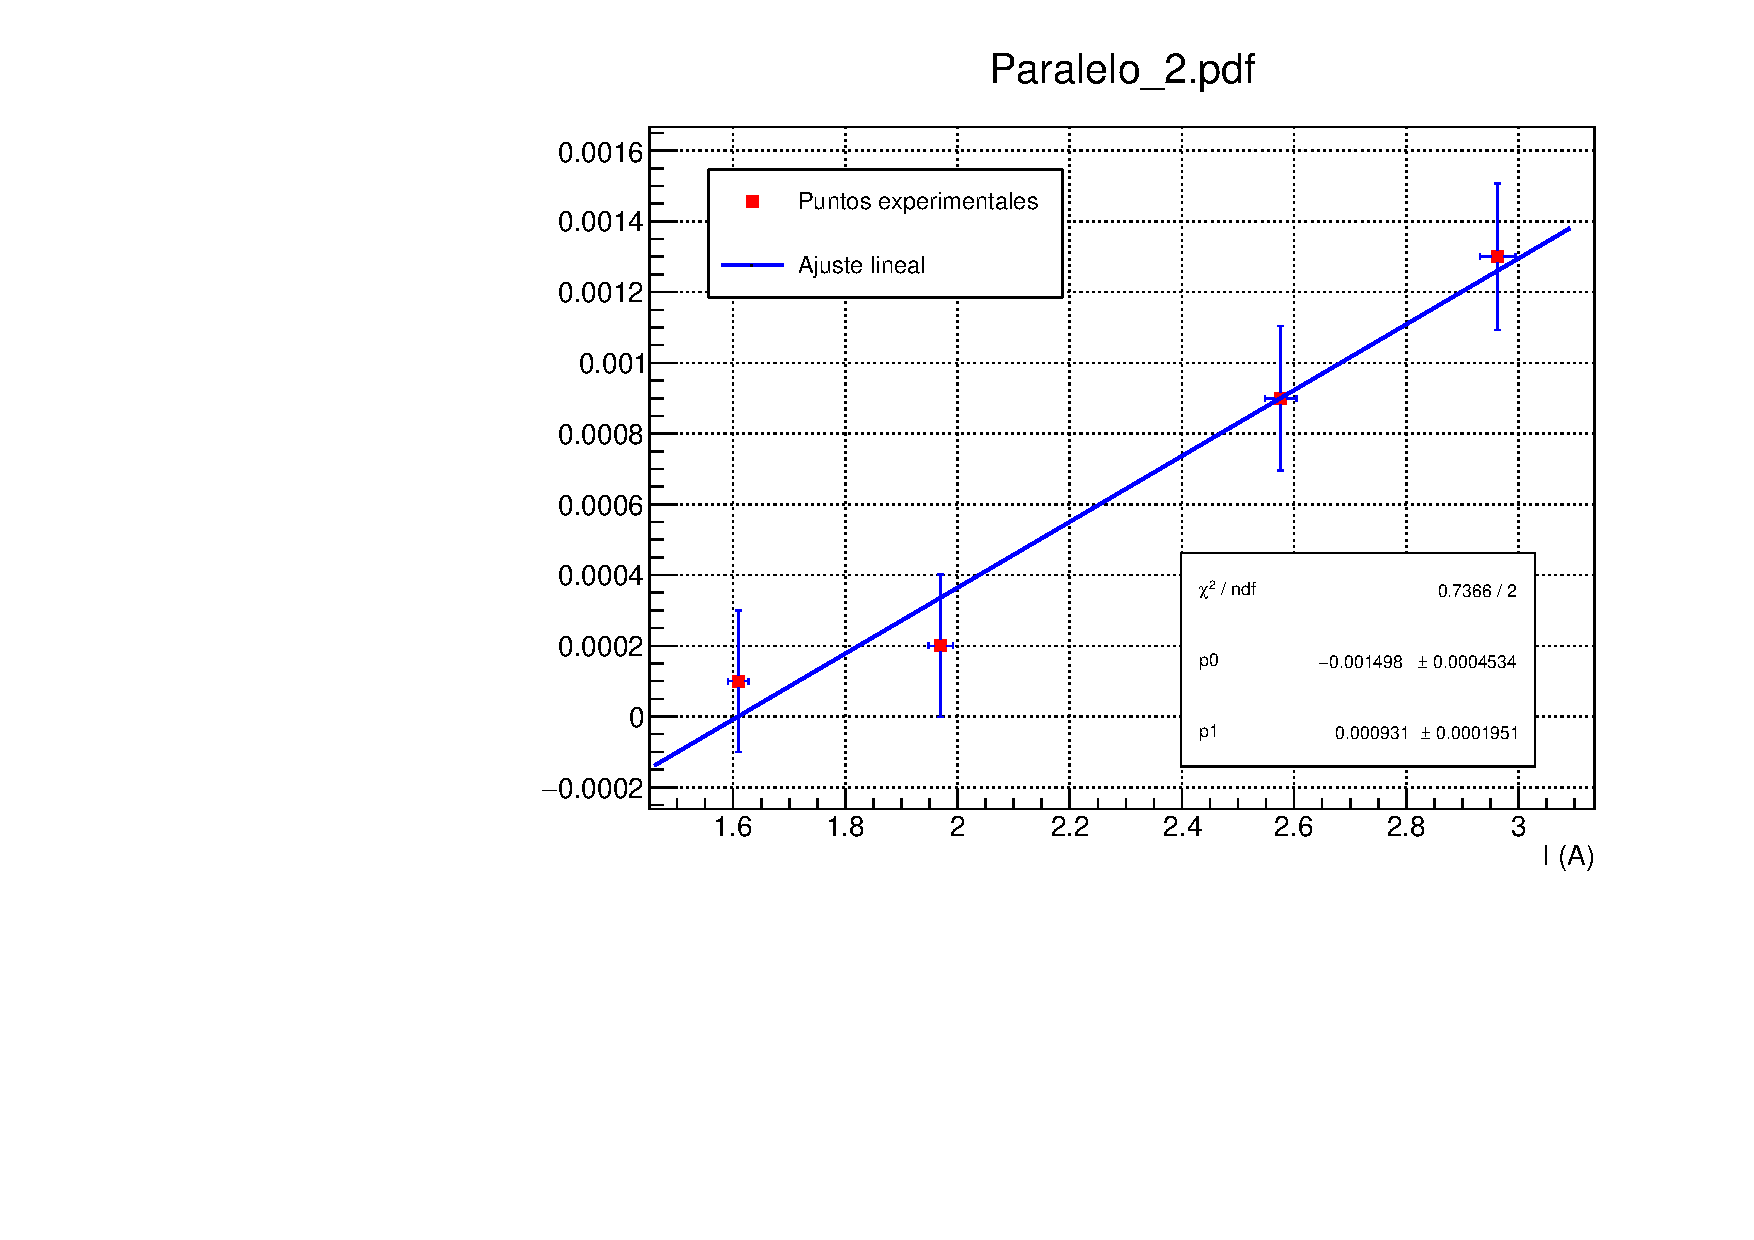
\includegraphics[width=1.05\linewidth]{Programas/Paralelo_2.pdf}
\end{subfigure}
\end{figure}
\begin{figure}[h!]\centering
\begin{subfigure}[b]{0.49\textwidth}
	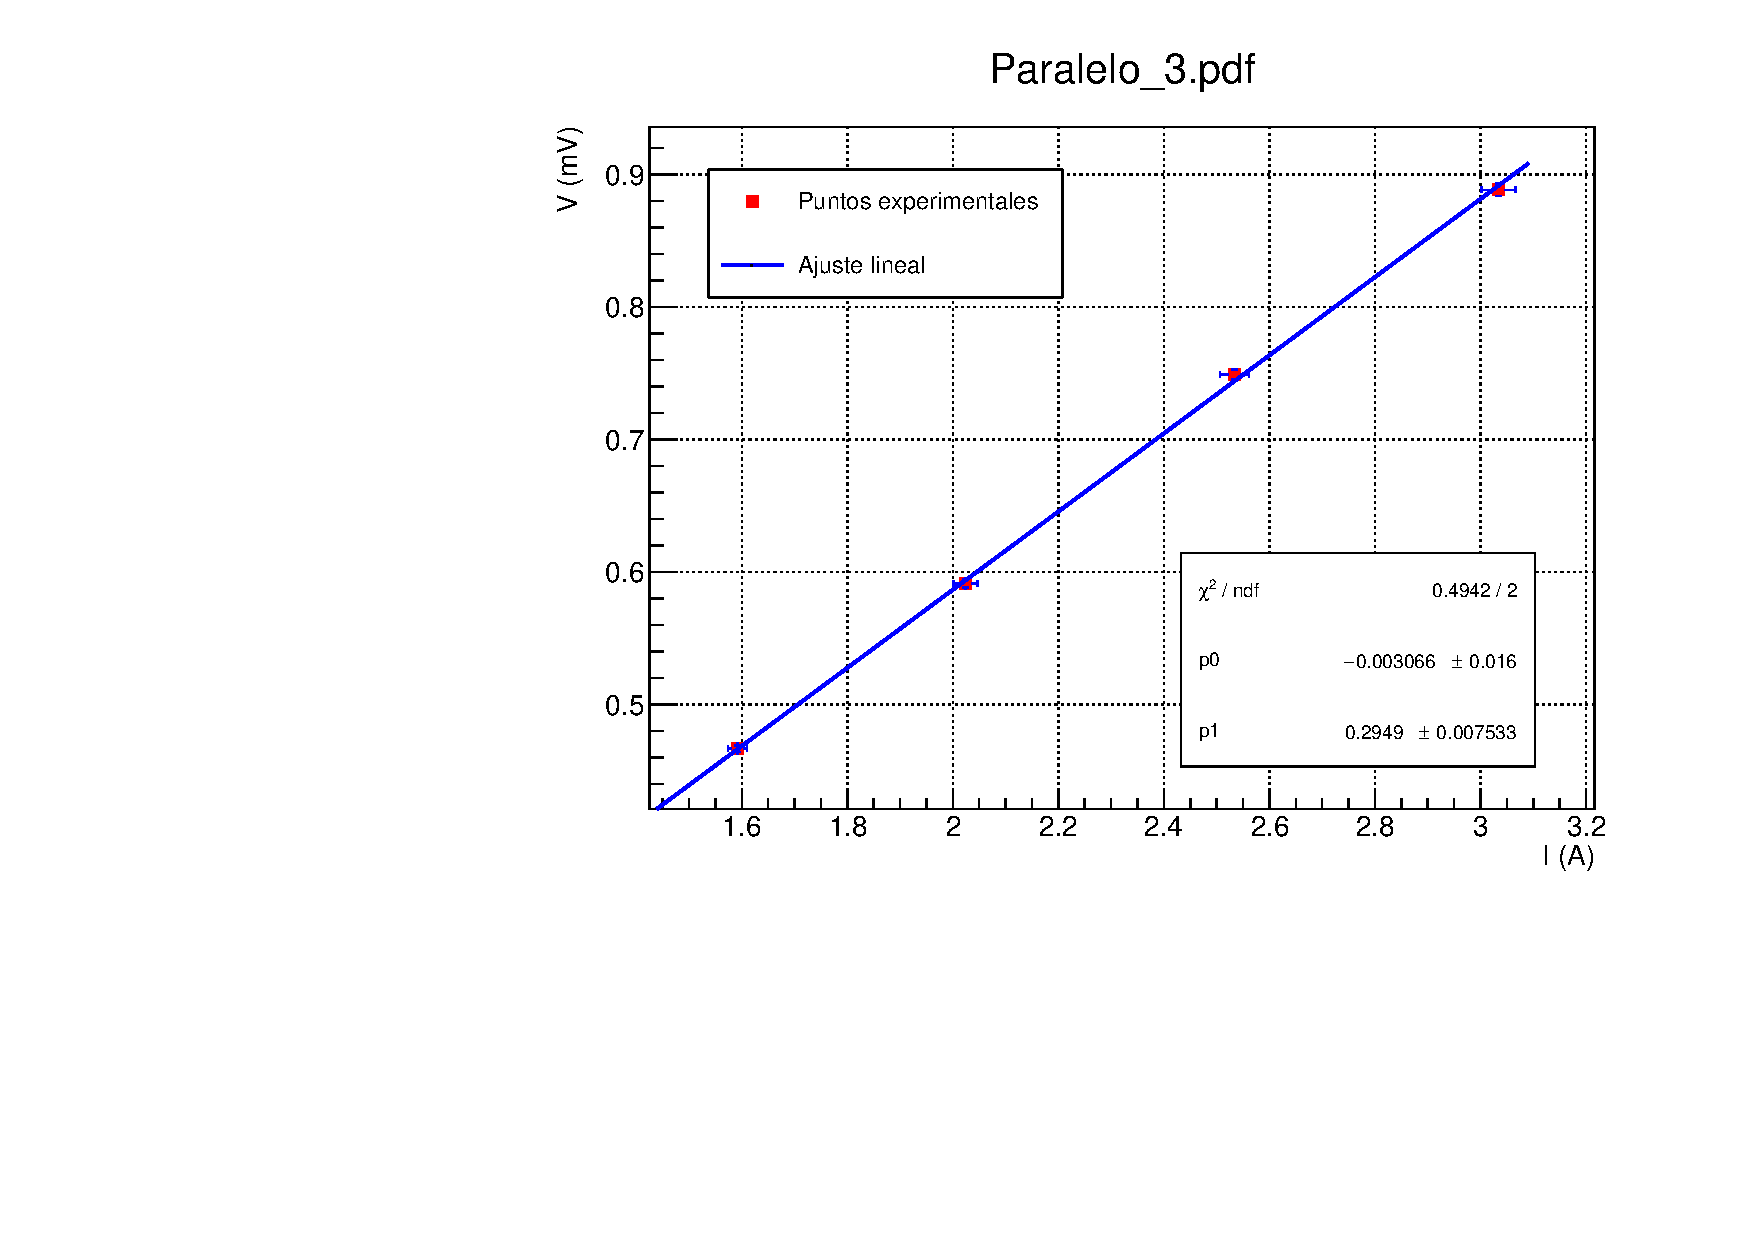
\includegraphics[width=1.05\linewidth]{Programas/Paralelo_3.pdf}
\end{subfigure} \hfill
\begin{subfigure}[b]{0.49\textwidth}
	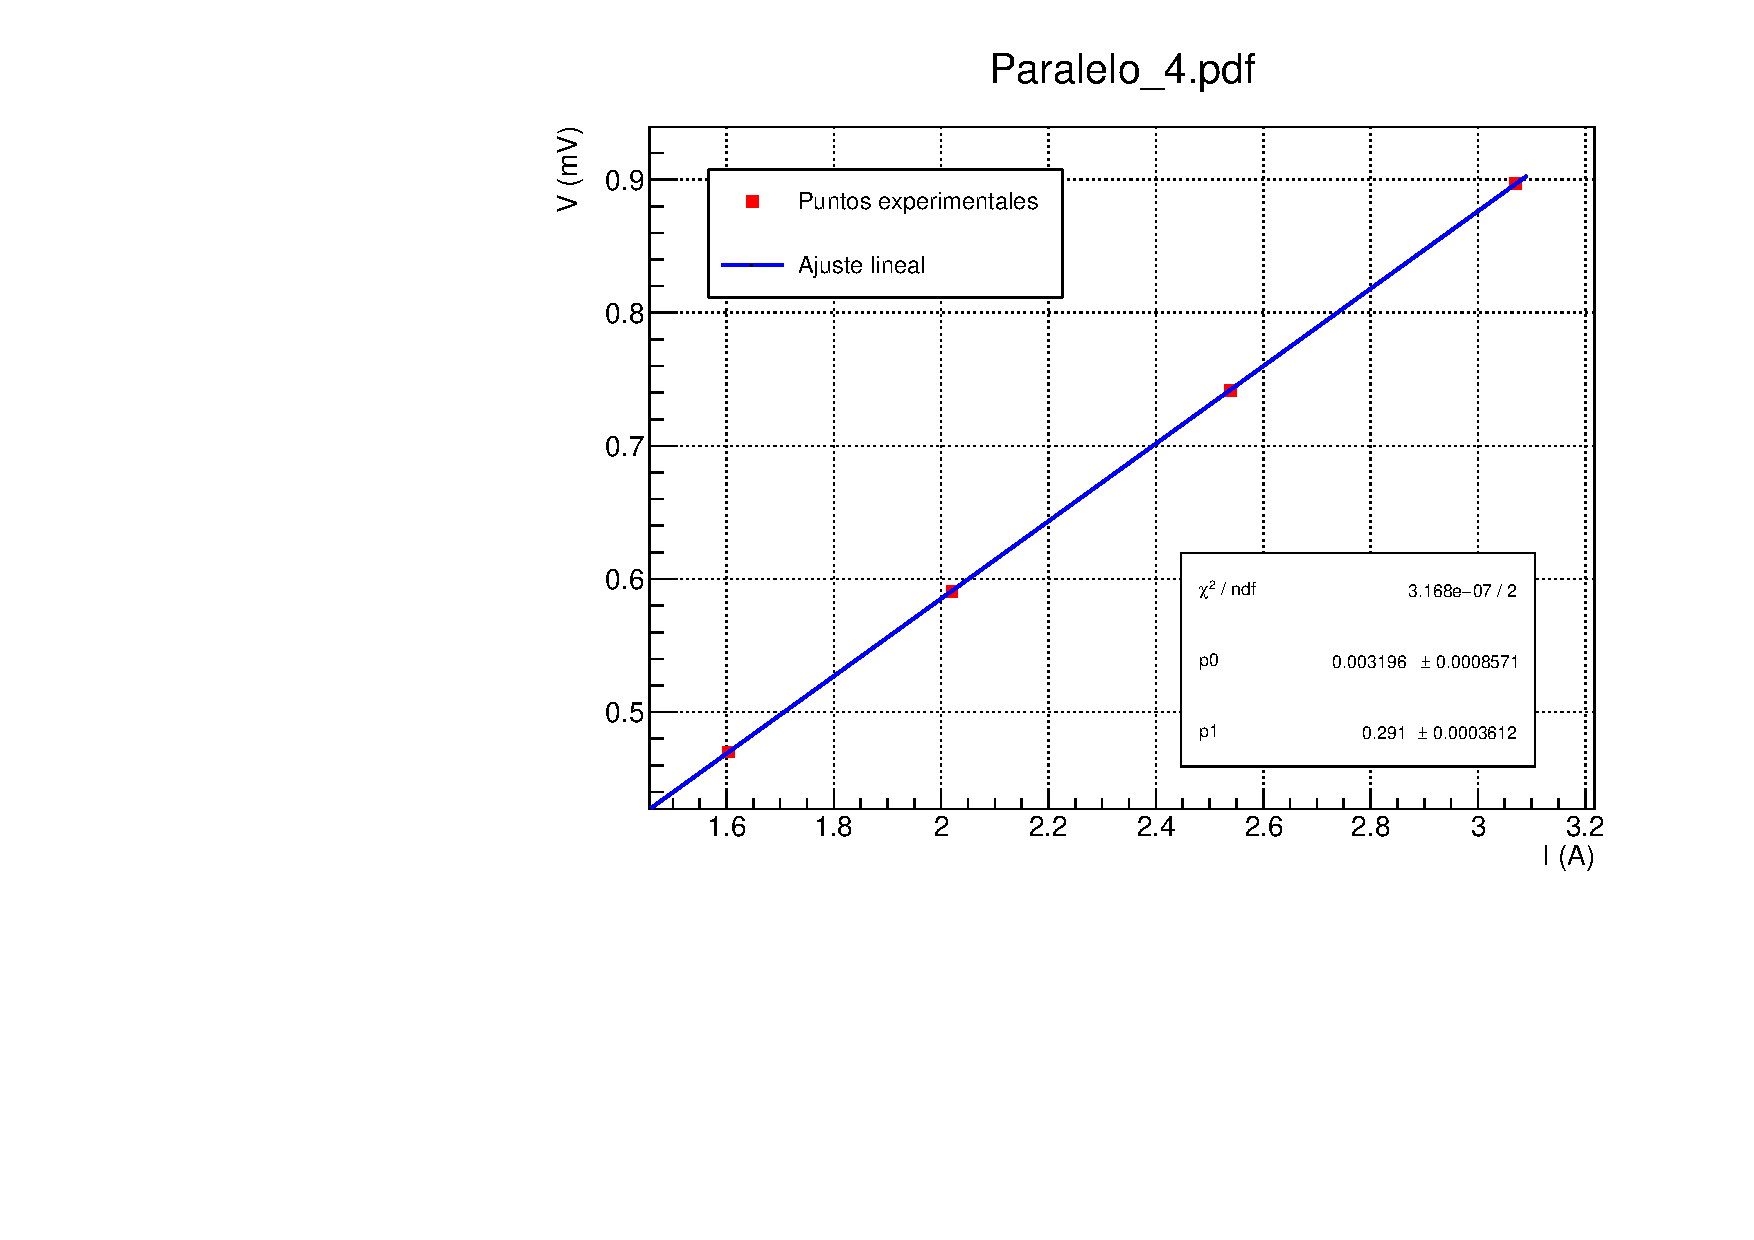
\includegraphics[width=1.05\linewidth]{Programas/Paralelo_4.pdf}
\end{subfigure}
\end{figure}


\subsection{Valores de la resistividad}

\section{Repetición de resultados; modelización de los terminales}

\section{Simulación}



\appendix

\section{Datos}

\section{Imágenes}



\end{document}